\documentclass[10pt]{article}
\usepackage[utf8]{inputenc}
\usepackage[T1]{fontenc}
\usepackage{graphicx}
\usepackage[export]{adjustbox}
\graphicspath{ {./images/} }
\usepackage{amsmath}
\usepackage{amsfonts}
\usepackage{amssymb}
\usepackage[version=4]{mhchem}
\usepackage{stmaryrd}

\title{S2l }


\author{Objectif\\
Vérifier le respect de l'exigence relative à la position d'équilibre du système}
\date{}


\begin{document}
\maketitle
\begin{center}
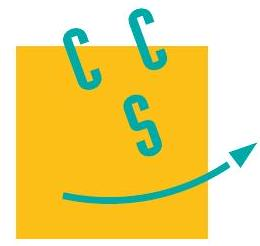
\includegraphics[max width=\textwidth]{2022_12_31_ed674c1a831ea1bff3a0g-01}
\end{center}

CONCOURS CENTRHLE•SUPÉLEC

R

\section{Stabilisateur vertical pour appareil photo}
\section{Contexte}
L'utilisation du mode vidéo, en haute définition sur les appareils photo réflex et légers, pose aux photographes le problème de la stabilisation de l'image car les vibrations engendrées y sont importantes et visibles. Des stabilisateurs installés à l'intérieur des appareils diminuent l'effet de ces vibrations mais ils restent très insuffisants pour assurer une bonne stabilisation notamment sur des sujets mobiles car ces systèmes ne sont efficaces que pour des temps de pose relativement longs. C'est pour cette raison que des systèmes de stabilisation externes ont été développés avec des supports et accessoires purement mécaniques ou motorisés.

\section{Nacelles gyrostabilisées}
Parmi les systèmes de stabilisation externes, les nacelles gyrostabilisées, installées sur une perche portée par les deux mains de l'utilisateur et sur lesquelles se fixe l'appareil photographique présentent l'avantage d'être légères, compactes et d'utilisation facile. Elles permettent de corriger les perturbations dues aux mouvements de l'utilisateur selon trois axes de rotations (figure 1). Néanmoins, elles ne permettent pas de réduire les perturbations verticales dues à la marche ou à la course de l'utilisateur.

\begin{center}
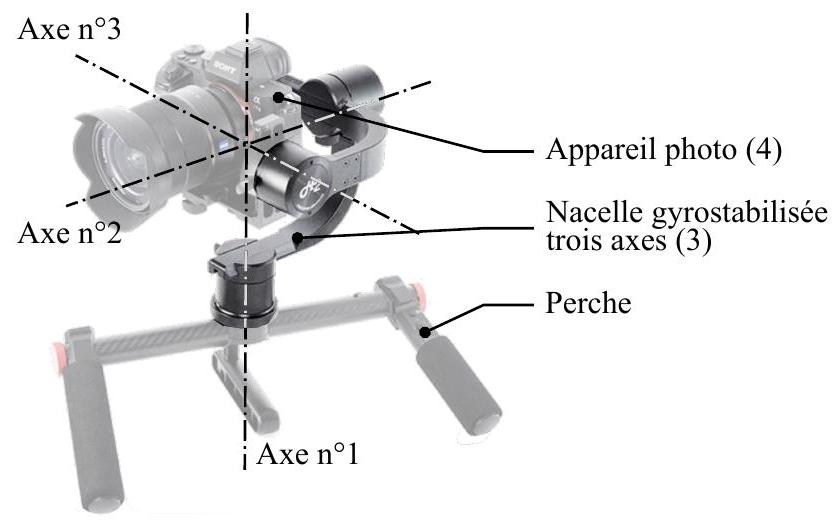
\includegraphics[max width=\textwidth]{2022_12_31_ed674c1a831ea1bff3a0g-01(1)}
\end{center}

Figure 1 Nacelle gyrostabilisée

\section{Stabilisateur vertical}
Pour maitriser les perturbations verticales dues à la marche ou la course des photographes, un constructeur commercialise un stabilisateur vertical à installer entre la perche et la nacelle gyrostabilisée (figure 2).

\begin{center}
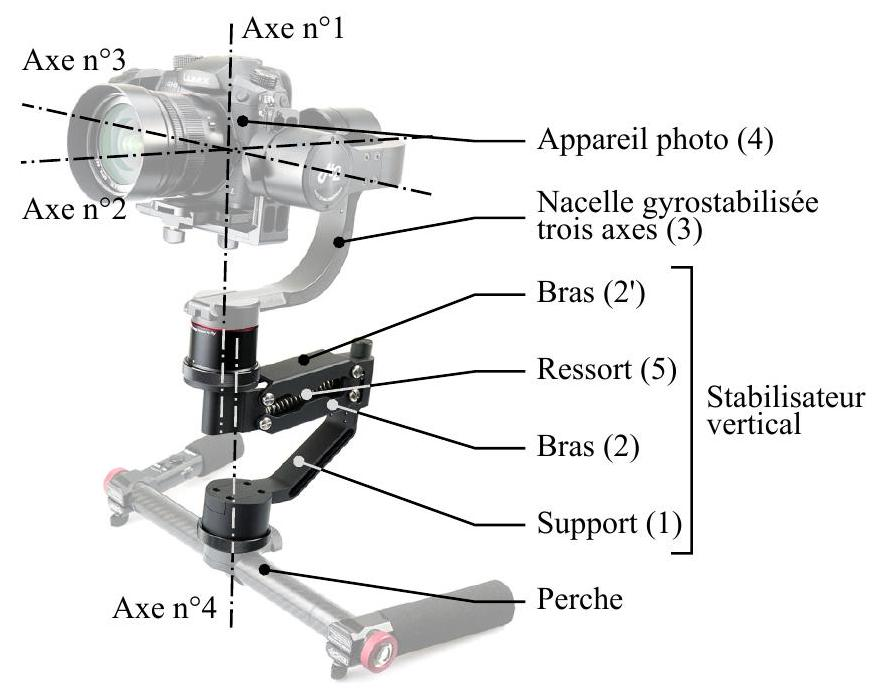
\includegraphics[max width=\textwidth]{2022_12_31_ed674c1a831ea1bff3a0g-01(2)}
\end{center}

Figure 2 Nacelle gyrostabilisée avec stabilisateur vertical

Une analyse du besoin des photographes a permis de documenter le cahier des charges fonctionnel dont un extrait est donné figure A du document réponse. Le cadre de ce sujet porte plus spécifiquement sur l'évaluation des solutions retenues pour satisfaire les objectifs de maitrise de la position d'un appareil photo à l'équilibre et en mouvement. Le sujet est décomposé en quatre parties :

\begin{itemize}
  \item dans la partie I, une analyse des mouvements de marche et de course d'un utilisateur est effectuée et les critères chiffrés de l'exigence relative à la position de l'appareil photo en mouvement sont justifiés ;

  \item la partie II porte sur la vérification du respect de l'exigence relative à la position à l'équilibre de l'appareil photo ;

  \item en partie III, une étude dynamique met en évidence la nécessité d'ajouter une commande active au système pour assurer le respect de l'exigence relative à la position en mouvement de l'appareil photo ;

  \item la partie IV porte sur la conception de la commande active du système en vue d'assurer la maitrise de la position de l'appareil photo avec le niveau de précision requis par le cahier des charges.

\end{itemize}

\section*{I Analyse du mouvement de l'utilisateur et justification du cahier des charges }
Pour réduire les perturbations verticales de l'appareil photo, la solution retenue est de filtrer les mouvements de translation verticale de la perche dont les fréquences sont précisées dans le cahier des charges (figure A). Pour justifier ces performances, on réalise des captures du mouvement vertical d'une perche tenue des deux mains par un utilisateur qui se déplace sur un sol plat.

Cette capture de mouvement est réalisée à partir d'un système optoélectronique dont le principe est le suivant : des caméras projettent une lumière dans le spectre infrarouge et détectent la lumière réfléchie par des marqueurs réfléchissants placés sur l'utilisateur. À partir des focales des caméras, de leur position et de leur orientation, il est possible de reconstruire, à chaque instant, par triangulation, la position spatiale des marqueurs et d'en déduire le mouvement vertical des mains, en retenant la valeur moyenne de la position verticale des deux mains. Les graphes des enregistrements de deux passages, marche et course, sont donnés ainsi que leur analyse spectrale (figure 3). Le contenu spectral est estimé en utilisant un enregistrement sur une durée limitée et la relation utilisée permet d'obtenir directement les amplitudes des différentes composantes harmoniques. Le calcul du spectre est réalisé pour un ensemble de fréquences choisi selon une distribution linéaire.
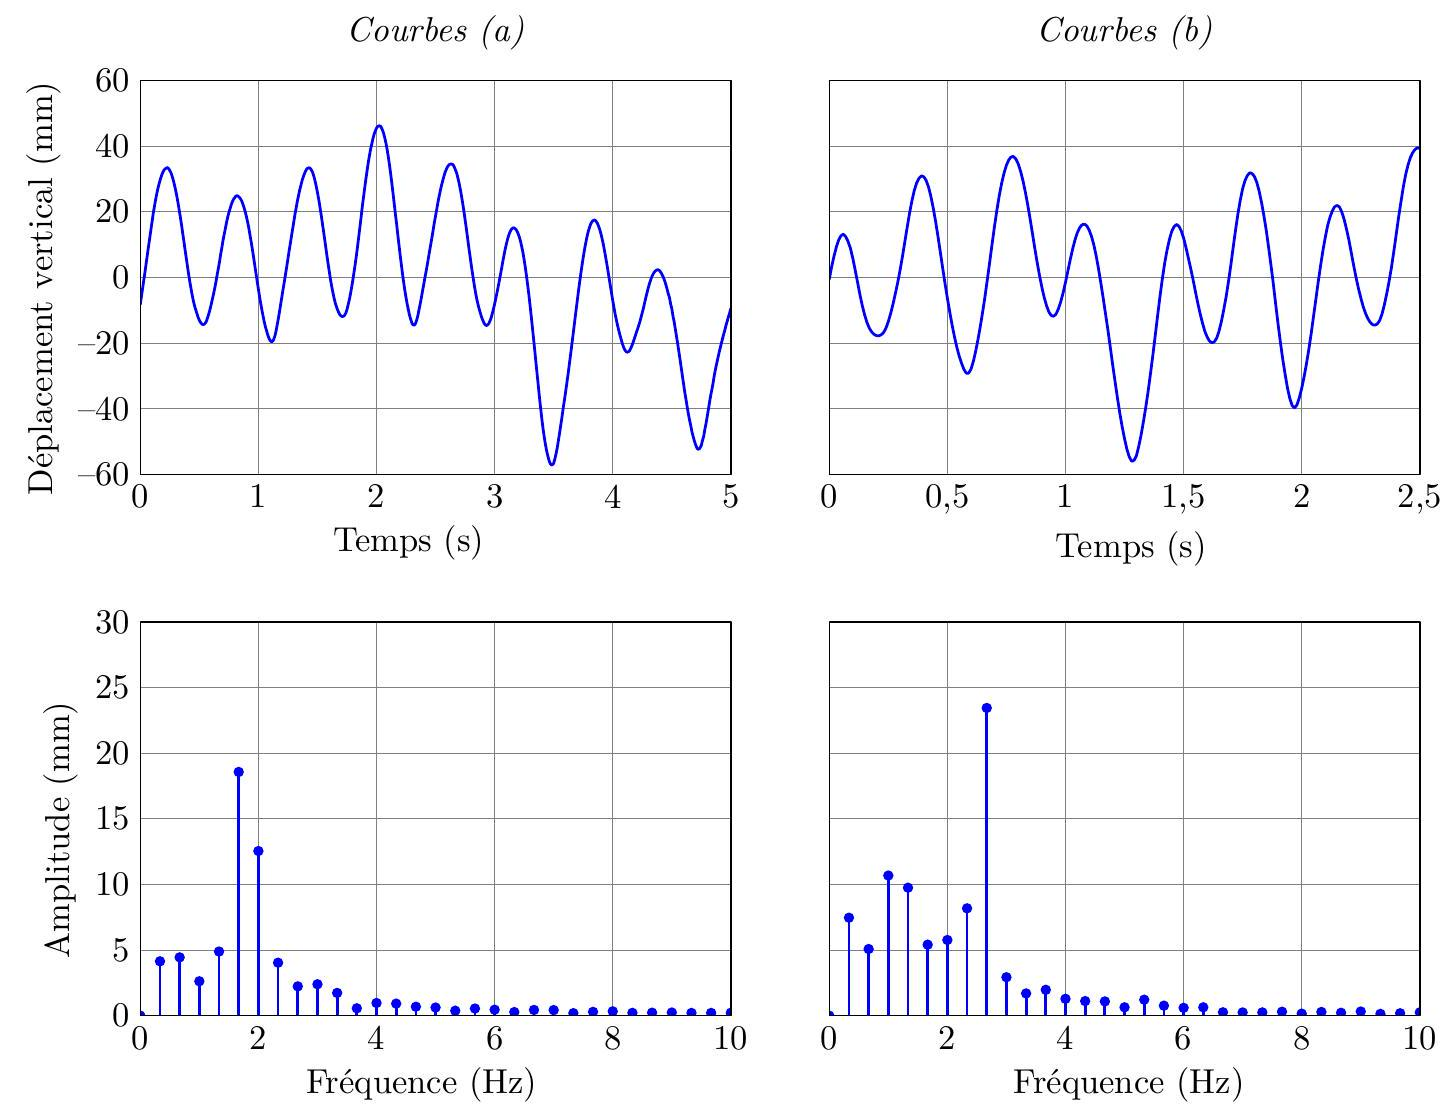
\includegraphics[max width=\textwidth, center]{2022_12_31_ed674c1a831ea1bff3a0g-02}

Figure 3 Représentations temporelle et spectrale du déplacement vertical des mains de l'utilisateur lors de la capture du mouvement Q 1. Associer chacune des courbes (a) ou (b) à l'enregistrement du mouvement pendant la marche ou la course de l'utilisateur. Il est conseillé d'analyser les caractéristiques de l'harmonique de plus grande amplitude.

Q 2. Proposer une méthode de filtrage pour atténuer les perturbations dues à la marche ou à la course de l'utilisateur tout en conservant les mouvements de translation verticale souhaités.

\section*{II Vérification du respect de l'exigence relative à la position d'équi- libre }
Le cahier des charges précise que le stabilisateur peut être utilisé avec des appareils photo de masse comprise entre 0,350 kg et 1,550 kg (figure A). L'objectif de cette partie est de vérifier que la conception est assez robuste vis-à-vis du facteur de masse de l'appareil photo pour satisfaire l'exigence $1.1$ relative à la position d'équilibre du système.

\begin{center}
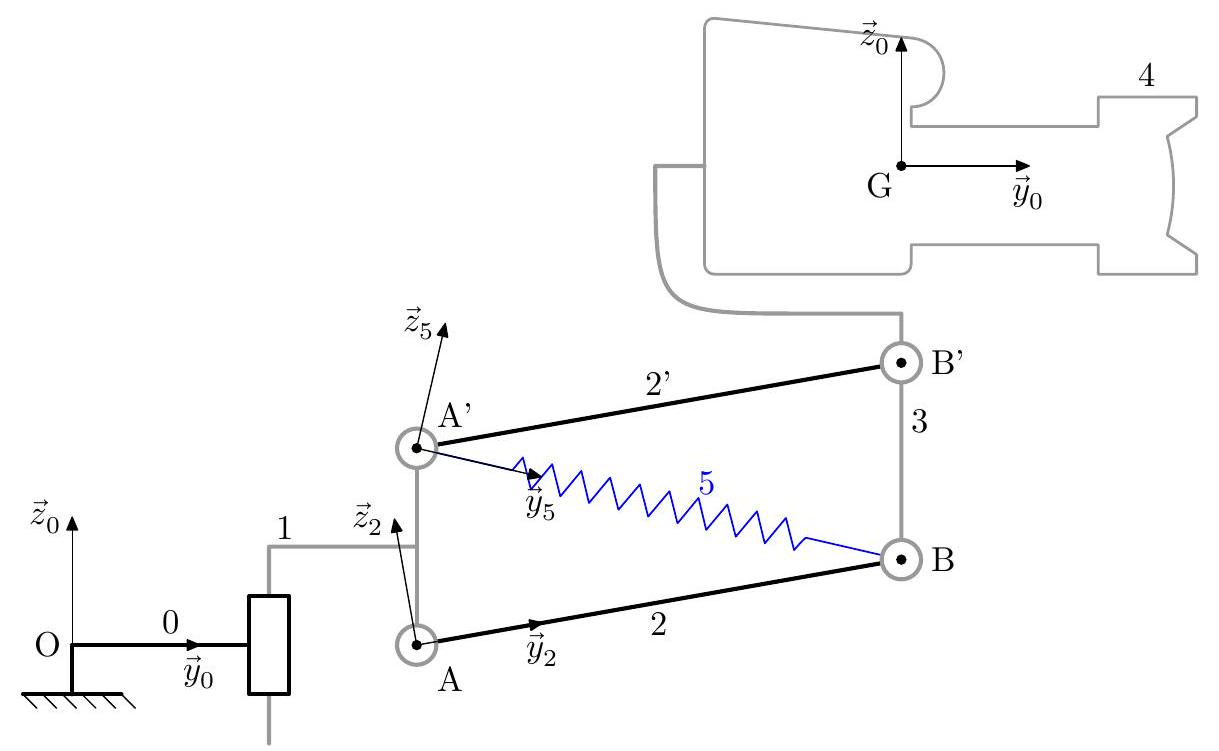
\includegraphics[max width=\textwidth]{2022_12_31_ed674c1a831ea1bff3a0g-03}
\end{center}

Figure 4 Schéma cinématique plan et paramétrage du mécanisme

Le mécanisme étudié dont la modélisation retenue est donnée (figure 4) est principalement constitué de quatre solides $\left\{(1),(2),\left(2^{\prime}\right),(3)\right\}$ formant un parallélogramme et guidés deux à deux en rotation par des liaisons modélisées par des pivots aux points A, A', B et B'. La nacelle gyrostabilisée est schématisée par la barre (3). Le support (1), faisant l'objet d'une liaison encastrement avec la perche, est supposé être en mouvement de translation par rapport au sol (0) autorisé par une glissière fictive. Ce modèle est paramétré par:

\begin{itemize}
  \item le repère terrestre $\mathcal{R}_{0}\left(\mathrm{O}, \vec{x}_{0}, \vec{y}_{0}, \vec{z}_{0}\right)$ supposé galiléen avec $\vec{z}_{0}$ vertical ascendant ;

  \item le repère $\mathcal{R}_{1}\left(\mathrm{~A}, \vec{x}_{0}, \vec{y}_{0}, \vec{z}_{0}\right)$ lié au support (1) avec $\overrightarrow{\mathrm{OA}}=y_{A} \vec{y}_{0}+z_{\text {pert }} \vec{z}_{0}$;

  \item le repère $\mathcal{R}_{2}\left(\mathrm{~A}, \vec{x}_{0}, \vec{y}_{2}, \vec{z}_{2}\right)$ lié au bras (2) avec $\alpha=\left(\vec{y}_{0}, \vec{y}_{2}\right)=\left(\vec{z}_{0}, \vec{z}_{2}\right)$;

  \item le repère $\mathcal{R}_{2}^{\prime}\left(\mathrm{A}^{\prime}, \vec{x}_{0}, \vec{y}_{2}, \vec{z}_{2}\right)$ lié au bras (2') avec $\overrightarrow{\mathrm{AA}^{\prime}}=l \vec{z}_{0}$;

  \item le repère $\mathcal{R}_{3}\left(\mathrm{~B}, \vec{x}_{0}, \vec{y}_{0}, \vec{z}_{0}\right)$ lié à la nacelle gyrostabilisée (3) et à l'appareil photo (4) liés rigidement entre eux avec $\overrightarrow{\mathrm{AB}}=L \vec{y}_{2}$. Le centre d'inertie de l'ensemble $\{(3)+(4)\}$ est noté $\mathrm{G}$, avec $\overrightarrow{\mathrm{BG}}=y_{G} \vec{y}_{0}+z_{G} \vec{z}_{0} ;$

  \item le repère $\mathcal{R}_{5}\left(\mathrm{~A}^{\prime}, \vec{x}_{0}, \vec{y}_{5}, \vec{z}_{5}\right)$ est défini tel que $\overrightarrow{\mathrm{A}^{\prime} \mathrm{B}}=L_{r} \vec{y}_{5}$ avec $\beta=\left(\vec{y}_{0}, \vec{y}_{5}\right)=\left(\vec{z}_{0}, \vec{z}_{5}\right)$.

\end{itemize}

La plage de fonctionnement du mécanisme est limitée par la géométrie des bras (2) et (2') avec $\alpha \in\left[-35^{\circ}, 45^{\circ}\right.$, $l=25 \mathrm{~mm}, L=52 \mathrm{~mm}, y_{G}=5 \mathrm{~mm}$ et $z_{G}=200 \mathrm{~mm}$.

Le ressort de traction (5) de raideur $K_{r}$ et de longueur à vide $L_{r 0}$ possède une tension initiale $F_{r 0}$ lorsque $L_{r}=L_{r 0}$. Il est relié d'une part au support (1) et d'autre part au solide (3) aux points d'ancrage respectivement A' et B.

Pour cette étude :

\begin{itemize}
  \item la nacelle gyrostabilisée (3) et l'appareil photo (4) sont considérés comme formant un seul solide ;

  \item la masse et les inerties des solides sont négligées mis à part pour l'ensemble constitué de la nacelle gyrostabilisée (3) et de l'appareil photo (4) de masse $m_{34}=m_{3}+m_{4}$ avec $m_{3}=1,250 \mathrm{~kg}$ la masse de la nacelle gyrostabilisée (3) et $m_{4}$ la masse de l'appareil photo (4). La référence retenue pour décrire la position de l'appareil photo est le centre d'inertie $\mathrm{G}$ de l'ensemble constitué de la nacelle gyrostabilisée (3) et de l'appareil photo (4) dans le repère $\mathcal{R}_{0}$.

\end{itemize}

Dans cette partie, l'étude est conduite avec les hypothèses suivantes :

\begin{itemize}
  \item les quatre liaisons pivots et la liaison glissière sont parfaites ;

  \item la modélisation est plane ;

  \item il n'y pas de perturbation $\left(z_{\text {pert }}=0\right)$.

\end{itemize}

Q 3. Exprimer les coordonnées du centre d'inertie $\mathrm{G}$ dans le repère $\mathcal{R}_{0}$ en fonction de l'angle $\alpha$ et des paramètres géométriques du système.

Q 4. En utilisant une fermeture géométrique, donner l'expression de l'angle $\beta$ en fonction de l'angle $\alpha$ et des paramètres géométriques $L$ et $l$ du système.

Q 5. Exprimer la longueur $L_{r}$ du ressort de traction (5) en fonction de l'angle $\alpha$ et des paramètres géométriques du système.

\section{II.A - Vérification de l'exigence relative à la plage de fonctionnement}
L'action mécanique du ressort de traction (5) sur la nacelle gyrostabilisée (3) est modélisée par le torseur $\left\{\mathcal{F}_{5 \rightarrow 3}\right\}:$

$$
\left\{\mathcal{F}_{5 \rightarrow 3}\right\}=\left\{\begin{array}{c}
F_{r} \vec{y}_{5} \\
\overrightarrow{0}
\end{array}\right\}_{\mathrm{B}} .
$$

Q 6. Exprimer la composante de résultante d'action mécanique $F_{r}$ en fonction de l'angle $\alpha$, des paramètres géométriques du système et des paramètres du ressort.

Q 7. Déterminer la direction des actions mécaniques de liaison exercées par le bras (2) sur la nacelle (3) et par le bras (2') sur la nacelle (3).

Q 8. Afin de déterminer la position d'équilibre de l'ensemble $\{(3)+(4)\}$, proposer sans calcul, une démarche claire qui permette d'exprimer l'effort nécessaire du ressort de traction (5) sur la nacelle gyrostabilisée (3).

Q 9. Exprimer l'équation scalaire traduisant l'équilibre du mécanisme en fonction des angles $\alpha$, $\beta$, de la masse $m_{34}$ et de la composante de résultante d'action mécanique $F_{r}$.

À partir des relations déterminées précédemment, deux fonctions beta(alpha) et effort\_ressort(alpha) qui renvoient respectivement la valeur de l'angle $\beta$ et la valeur de la composante de résultante d'action mécanique $F_{r}$ sont implantées en Python. La bibliothèque numpy a été importée sous le nom abrégé np. Les variables globales $\mathrm{g}$ et $\mathrm{m} 3$ fournissent respectivement la valeur de l'accélération de la pesanteur terrestre et la valeur de la masse de la nacelle gyrostabilisée (3). Les positions d'équilibre pour différentes valeurs de la masse $m_{4}$ sont alors obtenues par une méthode de recherche de zéro par dichotomie.

Q 10. Écrire en Python une fonction, fonction\_equilibre(m4, alpha), qui renvoie zéro lorsque, pour une valeur de masse $m_{4}$ de l'appareil photo donnée, la valeur de l'angle $\alpha$ vaut l'angle d'équilibre recherché.

Une fonction angle\_equilibre(m4) qui renvoie la valeur de l'angle $\alpha=\alpha_{0}$ correspondant à la position d'équilibre avec une méthode de recherche de zéro par dichotomie est implantée en Python. La courbe obtenue à partir de la fonction angle\_equilibre(m4) représentant l'angle d'équilibre $\alpha_{0}$ en fonction de la masse de l'appareil photo $m_{4}$ est donnée (figure 5).

Q 11. En donnant les valeurs des angles d'équilibre pour les deux valeurs extrêmes de masse, vérifier le respect de l'exigence 1.1.1. relative à la plage de fonctionnement.

\section{II.B - Vérification de l'exigence relative au mouvement de l'appareil photo autour des positions d'équilibre possibles}
Q 12. En étudiant le comportement du système autour des deux positions d'équilibre extrêmes, vérifier le respect de l'exigence 1.1.2. de l'appareil photo autour des positions d'équilibre possibles. Conclure sur le respect de l'exigence 1.1.

\begin{center}
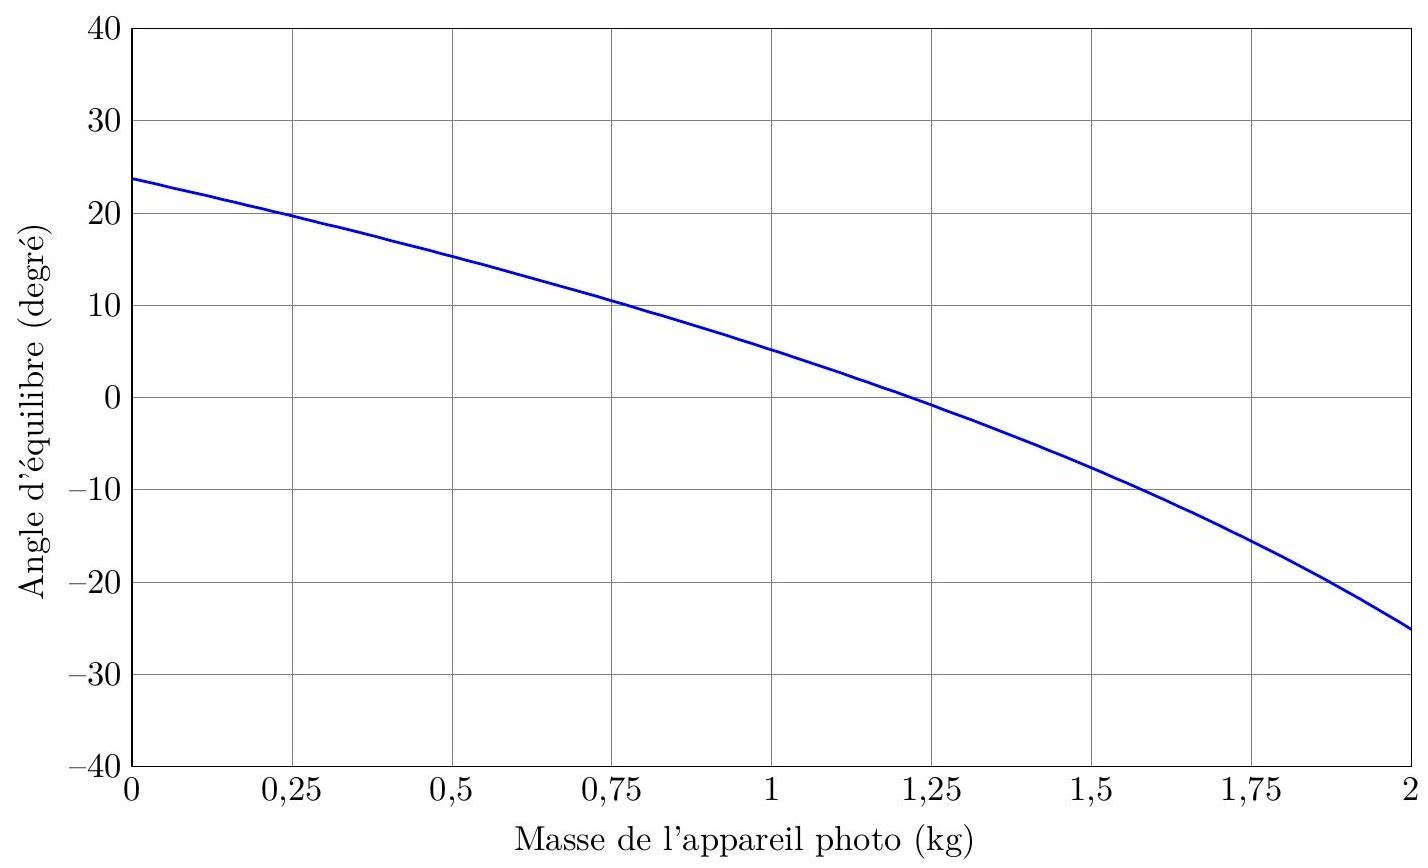
\includegraphics[max width=\textwidth]{2022_12_31_ed674c1a831ea1bff3a0g-05}
\end{center}

Figure 5 Angle d'équilibre $\alpha_{0}$ en fonction de la masse de l'appareil photo $m_{4}$

\section*{III Détermination de la loi de mouvement du système perturbé }
\begin{abstract}
Objectif Élaborer le modèle dynamique et déterminer la loi de mouvement du système perturbé afin de mettre en évidence la nécessité d'ajouter une commande active au système pour assurer le respect de l'exigence 1.2. relative à la position en mouvement du cahier des charges.
\end{abstract}

Dans cette partie, l'étude est conduite avec les hypothèses suivantes :

\begin{itemize}
  \item les quatre liaisons pivots et la liaison glissière sont parfaites ;

  \item la modélisation est plane ;

  \item le système est perturbé par l'utilisateur au niveau de la glissière (figure 4) et cette perturbation est modélisée par une fonction sinusoïdale $z_{\text {pert }}(t)=Z_{0} \sin (\omega t)$ avec l'amplitude $Z_{0}$ et la pulsation $\omega$ constantes ;

  \item à l'instant initial de cette étude, la nacelle gyrostabilisée (figure 4) est à l'équilibre.

\end{itemize}

\section{III.A - Détermination de la loi de mouvement}
Q 13. En isolant l'ensemble constitué de la nacelle gyrostabilisée (3) et de l'appareil photo (4) (formant un seul solide) et en traduisant une équation scalaire issue du principe fondamental de la dynamique, donner l'équation différentielle traduisant la loi de mouvement du système. Écrire l'équation différentielle sous la forme

$$
\ddot{\alpha}=C_{1} \ddot{z}_{\text {pert }} \cos \alpha+C_{2} \cos \alpha+C_{3} F_{r} \sin (\beta-\alpha)
$$

en précisant l'expression des trois constantes $C_{1}, C_{2}$ et $C_{3}$ en fonction de $m_{34}, L$ et $g$.

L'équation différentielle traduisant la loi de mouvement du système est du second ordre. Pour résoudre numériquement une telle équation différentielle, elle peut être réécrite sous la forme d'une équation différentielle vectorielle du premier ordre. On définit pour cela, le vecteur $A(t)$ par

$$
A(t)=\left(\begin{array}{c}
\alpha(t) \\
\dot{\alpha}(t)
\end{array}\right) .
$$

L'équation différentielle du mouvement peut alors se mettre sous la forme du problème de Cauchy

$$
\dot{A}(t)=\frac{\mathrm{d} A(t)}{\mathrm{d} t}=\left(\begin{array}{c}
\dot{\alpha}(t) \\
\ddot{\alpha}(t)
\end{array}\right)=f(A(t), t) .
$$

dont une solution peut être calculée à l'aide de la fonction integrate. odeint de la bibliothèque Python scipy dont le mode d'emploi est précisé dans le document réponse. $\mathrm{AO}=.$. . \# à définir

$\mathrm{t}=\mathrm{np}$.arange $(0,4,0.01)$

$A=$ scipy.integrate.odeint(equation\_dynamique, $A 0, t$ )

À partir des relations déterminées précédemment, les fonctions beta(alpha), effort\_ressort(alpha) et angle\_equilibre(m4) sont implantées en Python. Elles renvoient respectivement la valeur de l'angle $\beta$, la valeur de la composante de résultante d'action mécanique $F_{r}$ et la valeur de l'angle correspondant à la position d'équilibre. La bibliothèque numpy a été importée sous le nom abrégé np. Les variables globales C1, C2, C3, Z0 et w fournissent respectivement les valeurs des trois constantes $C_{1}, C_{2}$ et $C_{3}$, de l'amplitude $Z_{0}$ et la pulsation $\omega$.

Q 14. Écrire en Python une fonction equation\_dynamique $(A, t)$ qui renvoie le vecteur dérivé $\dot{A}(t)$ en fonction du vecteur A et la date t correspondante.

Q 15. Écrire l'instruction Python permettant de définir la condition initiale A0.

La résolution de l'équation différentielle permet d'obtenir l'évolution de l'angle $\alpha$ au cours du temps. Le déplacement vertical de l'appareil photo est déterminé à partir de cette solution et des relations déterminées précédemment.

\section{III.B - Validation expérimentale du modèle dynamique}
Pour valider le modèle dynamique, le stabilisateur vertical est soumis à une perturbation sinusoïdale $z_{\text {pert }}(t)=$ $Z_{0} \sin (\omega t)$. Les courbes expérimentales (figure 6 en bas) ainsi obtenues sont à comparer avec les solutions issues de la résolution de l'équation différentielle (figure 6 en haut).

Fréquence $1 \mathrm{~Hz}$
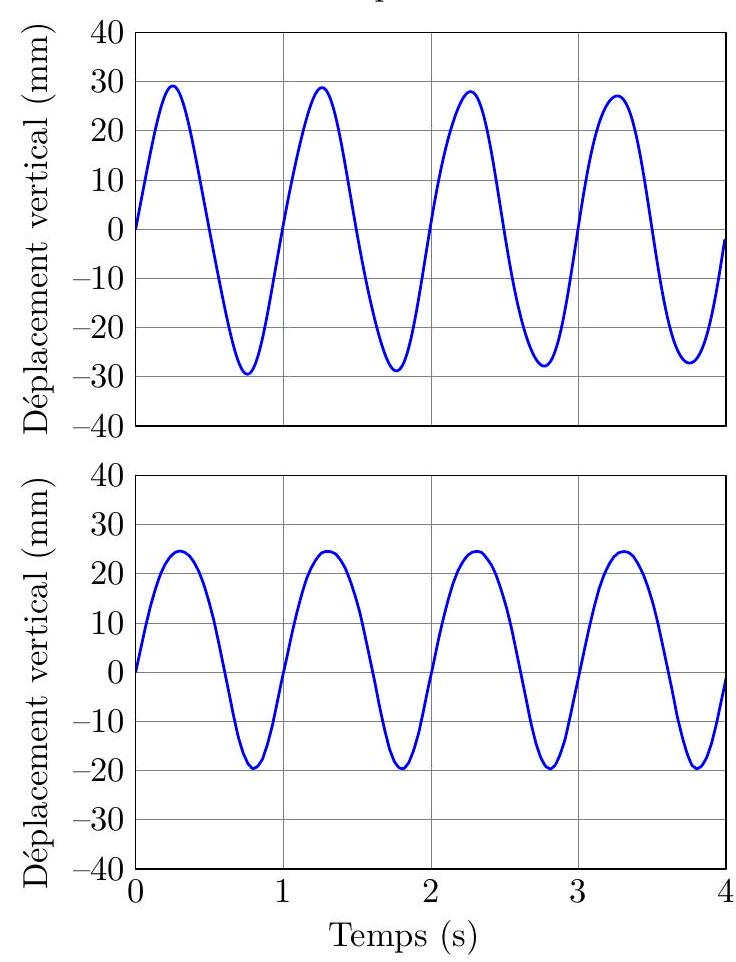
\includegraphics[max width=\textwidth, center]{2022_12_31_ed674c1a831ea1bff3a0g-06}

Fréquence $2 \mathrm{~Hz}$

\begin{center}
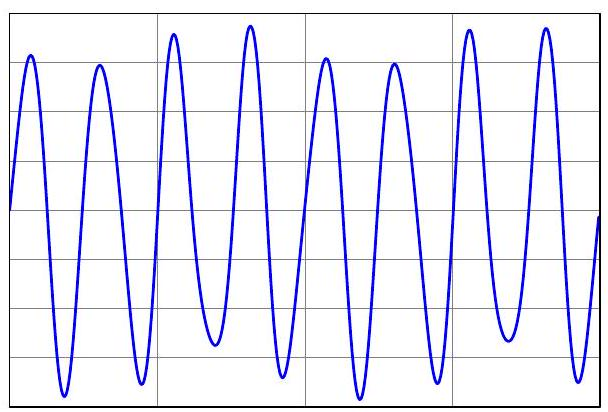
\includegraphics[max width=\textwidth]{2022_12_31_ed674c1a831ea1bff3a0g-06(1)}
\end{center}

Solutions de l'équation différentielle

\begin{center}
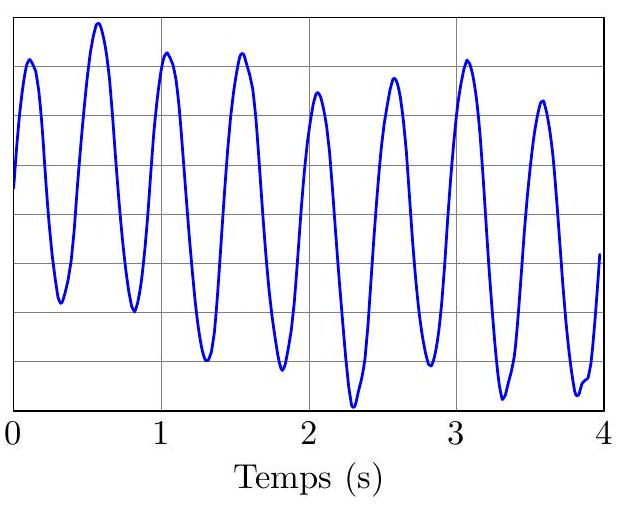
\includegraphics[max width=\textwidth]{2022_12_31_ed674c1a831ea1bff3a0g-06(2)}
\end{center}

Courbes

expérimentales

Figure 6 Déplacement vertical de l'appareil photo pour une perturbation d'amplitude $25 \mathrm{~mm}$ et de fréquences $1 \mathrm{~Hz}$ et $2 \mathrm{~Hz}$ avec une masse $m_{4}=1 \mathrm{~kg}$

Q 16. Comparer les performances mesurées et simulées (figure 6). Peut-on valider le modèle dynamique pour la vérification de l'exigence 1.2. relative à la position de l'appareil photo en mouvement ? Quel phénomène physique pourrait-on prendre en compte pour améliorer le modèle ?

\section{C - Conclusion}
Pour analyser le respect de l'exigence 1.2. relative à la position en mouvement, des simulations sont réalisées dans plusieurs configurations (figure 7).

Q 17. Conclure sur la satisfaction de l'exigence 1.2. relative à la position de l'appareil photo en mouvement à l'aide des résultats de simulation (figure 7).

Une modification des caractéristiques du ressort pourrait permettre de respecter l'exigence 1.2. relative à la position de l'appareil photo en mouvement. Néanmoins, cette modification impacterait le comportement du système à l'équilibre et ne permettrait plus de respecter l'exigence 1.1. relative à la position d'équilibre. Pour cette raison, une solution technique avec une commande active est présentée et étudiée dans la partie suivante.

$$
m_{4}=0,350 \mathrm{~kg}
$$

\begin{center}
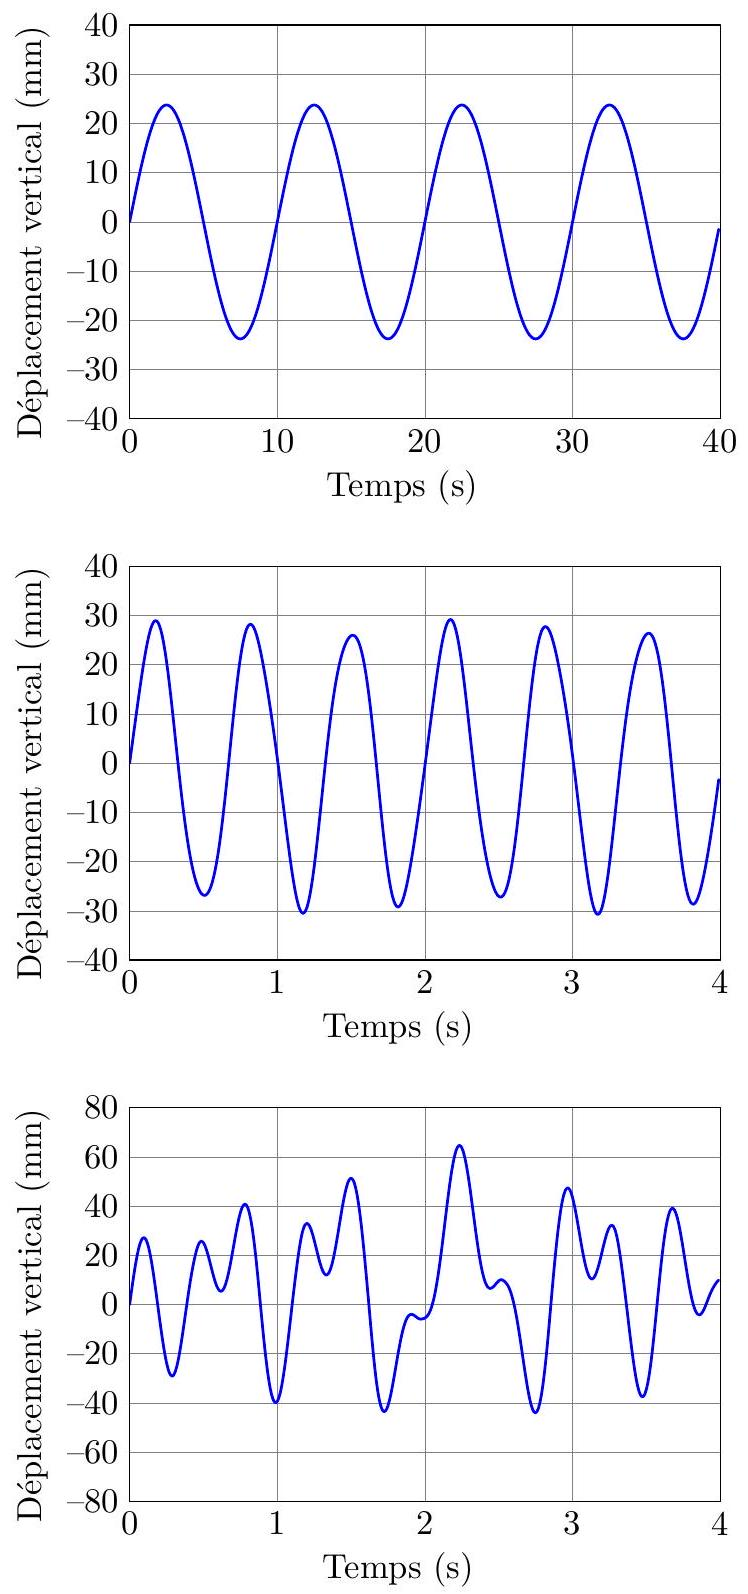
\includegraphics[max width=\textwidth]{2022_12_31_ed674c1a831ea1bff3a0g-07}
\end{center}

$m_{4}=1,550 \mathrm{~kg}$

\begin{center}
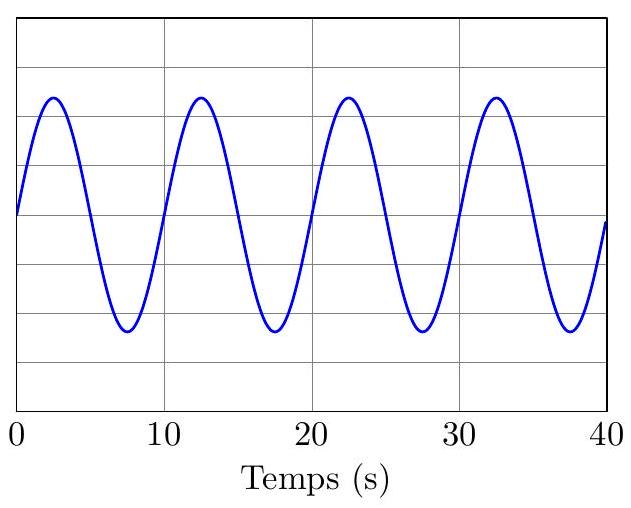
\includegraphics[max width=\textwidth]{2022_12_31_ed674c1a831ea1bff3a0g-07(1)}
\end{center}

Fréquence $0,1 \mathrm{~Hz}$
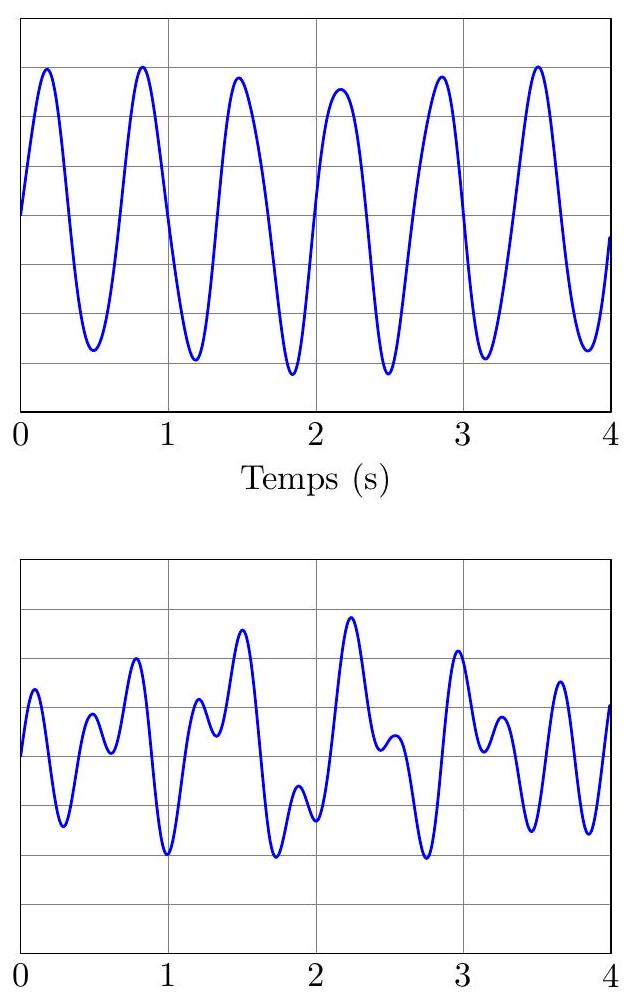
\includegraphics[max width=\textwidth, center]{2022_12_31_ed674c1a831ea1bff3a0g-07(2)}

Temps (s)

Fréquence $1,5 \mathrm{~Hz}$

Fréquence $2,8 \mathrm{~Hz}$

Figure 7 Simulations du déplacement vertical de l'appareil photo pour une perturbation d'amplitude $25 \mathrm{~mm}$ et de fréquences de $0,1 \mathrm{~Hz}, 1,5 \mathrm{~Hz}$ et $2,8 \mathrm{~Hz}$ avec des masses $m_{4}=0,350 \mathrm{~kg}$ et $m_{4}=1,550 \mathrm{~kg}$

\section*{IV Étude d'avant-projet d'une solution technique avec une com- mande active }
\textbackslash author\{

\begin{itemize}
  \item Objectif
\}
\end{itemize}

Modéliser la commande et déterminer le réglage du correcteur. Spécifier la motorisation.

Dans cette partie, la régulation en hauteur de l'ensemble constitué de la nacelle gyrostabilisée (3) et de l'appareil photo (4) est réalisée par un motoréducteur dont le stator est lié au support (1) et dont l'arbre de sortie entraine le bras (2) (figure 8). Le rendement de la chaine de motorisation est supposé parfait.

\begin{center}
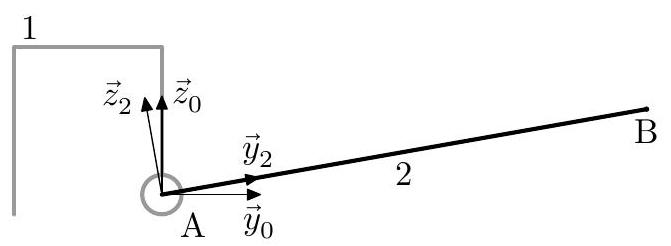
\includegraphics[max width=\textwidth]{2022_12_31_ed674c1a831ea1bff3a0g-07(3)}
\end{center}

Figure 8 Modèle simplifié Les grandeurs utilisées dans cette partie sont:

\begin{itemize}
  \item $C_{m}$ le moment du couple qui modélise l'action du moteur sur l'arbre d'entrée du réducteur ;

  \item $\omega_{m}$ la vitesse de rotation de l'arbre du moteur ;

  \item $C_{s}$ le moment du couple qui modélise l'action exercée par l'arbre de sortie du réducteur sur le bras (2) ;

  \item $\omega_{s}$ la vitesse de rotation de l'arbre de sortie du réducteur sur le bras (2);

  \item $N$ le rapport de transmission du réducteur avec $N=\omega_{m} / \omega_{s}=100$;

  \item $\alpha$ l'angle formé entre le bras (2) et le support (1) défini par $\alpha=\left(\vec{y}_{0}, \vec{y}_{2}\right)=\left(\vec{z}_{0}, \vec{z}_{2}\right)$;

  \item $F_{z}$ le modèle de la composante verticale de l'effort exercé sur l'ensemble constitué de la nacelle gyrostabilisée (3) et de l'appareil photo (4) dû au couple moteur ;

  \item $F_{p}$ le modèle de l'effort de perturbation, dû au poids de l'ensemble constitué de la nacelle gyrostabilisée (3) et de l'appareil photo (4) ;

  \item $C_{m}^{*}$ la consigne en couple sur la machine à courant continu ;

  \item $m_{34}$ la masse de l'ensemble constitué de la nacelle gyrostabilisée (3) et de l'appareil photo (4) ;

  \item $L$ la longueur du bras (2).

\end{itemize}

Un diagramme des exigences partiel du stabilisateur vertical avec la commande active est donné figure B du document réponse.

Les effets de masse et d'inertie du solide (2) sont négligeables devant les autres actions mises en jeu.

Q 18. En retenant le schéma simplifié (figure 8) et en modélisant par un glisseur dont la résultante est notée $\vec{F}_{2 \rightarrow 3}=F_{y} \vec{y}_{0}+F_{z} \vec{z}_{0}$ l'action mécanique exercée au point B par le bras (2) sur la nacelle gyrostabilisée (3), exprimer $C_{s}$ en fonction de $F_{z}, F_{y}, \alpha(t)$ et $L$.

En négligeant $F_{y}$ devant $F_{z}\left(F_{y} \approx 0\right)$ donner alors la relation entre $C_{m}, F_{z}, \alpha(t), L$ et $N$.

La machine à courant continu est modélisée comme un générateur de couple parfait, en particulier instantané. Le schéma-bloc de la boucle ouverte non corrigée du système est donné (figure 9) en faisant l'approximation des petits angles.

\begin{center}
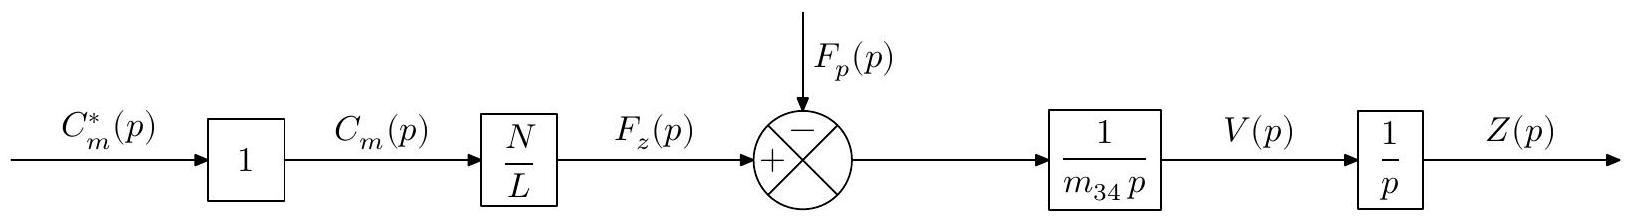
\includegraphics[max width=\textwidth]{2022_12_31_ed674c1a831ea1bff3a0g-08}
\end{center}

Figure 9 Schéma-bloc de la boucle ouverte non corrigée

Pour réaliser un asservissement, un comparateur forme la différence entre une consigne en position notée $\Delta Z^{*}(p)$ et une mesure de la hauteur $\Delta Z(p)$ de l'appareil photo renvoyée par un capteur. Cette différence est corrigée par un correcteur de fonction de transfert notée $C(p)$. En pratique, $\Delta Z(p)$ correspond à l'écart par rapport à une position de référence non présentée ici. Le capteur est modélisé par un gain unitaire. Le schéma-bloc d'asservissement est donné (figure 10).

\begin{center}
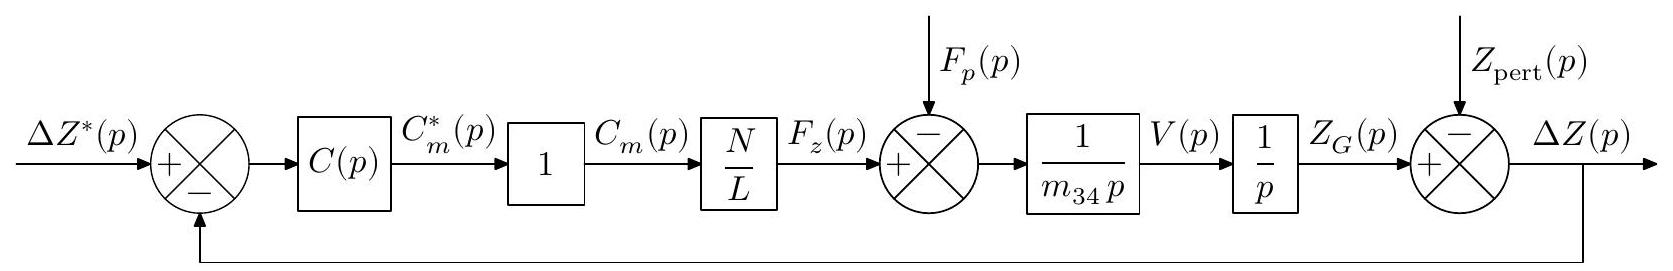
\includegraphics[max width=\textwidth]{2022_12_31_ed674c1a831ea1bff3a0g-08(1)}
\end{center}

Figure 10 Schéma-bloc de l'asservissement de position avec un correcteur $C(p)$

\section{IV.A - Choix et réglage du correcteur}
Dans cette sous-partie, après avoir mis en évidence la nécessité d'introduire un correcteur, l'objet est d'en régler les paramètres de manière à ce que les performances du système vérifient les exigences du cahier des charges (figure B).

Q 19. Montrer qu'un correcteur proportionnel $C(p)=K$ ne permet pas d'assurer la stabilité du système en boucle fermée.

Le correcteur retenu est de la forme

$$
C(p)=K\left(1+\frac{1}{T_{i} p}+T_{d} p\right) .
$$

En prenant $T_{i}=2 T$ et $T_{d}=T / 2$ on obtient le correcteur sous la forme

$$
C(p)=K \frac{(1+T p)^{2}}{2 T p} .
$$

On pourra utiliser dans la suite la relation approximative $T_{m, \mathrm{BF}} \omega_{c, 0 \mathrm{~dB}} \approx 3$, où $T_{m, \mathrm{BF}}$ désigne le temps du premier maximum en boucle fermée et $\omega_{c, 0 \mathrm{~dB}}$ est la pulsation de coupure à $0 \mathrm{~dB}$ en boucle ouverte.

La marge de phase minimale définie dans le cahier des charges est notée $\Delta \varphi$. On se place à la limite de la valeur exigée par le cahier des charges.

Q 20. En déduire les expressions respectives de l'argument et du module de la fonction de transfert du correcteur pour $\omega=\omega_{c, 0 \mathrm{~dB}}$ notées respectivement $\arg \left(C\left(\mathrm{j} \omega_{c, 0 \mathrm{~dB}}\right)\right)$ et $\left|C\left(\mathrm{j} \omega_{c, 0 \mathrm{~dB}}\right)\right|$ afin de vérifier l'exigence 2.3.1 relative à la stabilité de la commande active en fonction de $\omega_{c, 0 \mathrm{~dB}}, m_{34}, L, N$ et $\Delta \varphi$.

Q 21. Déterminer l'expression littérale du paramètre $T$ du correcteur. Effectuer l'application numérique.

Q 22. Déterminer l'expression littérale du paramètre $K$ du correcteur. Effectuer l'application numérique avec $m_{34}=2,8 \mathrm{~kg}, L=52 \mathrm{~mm}$ et $N=100$.

\section{IV.B - Spécification de l'actionneur}
Pour concevoir le prototype, il faut définir la chaine de motorisation. Dans ce but, l'actionneur est supposé asservi. La relation entre le couple de consigne et le couple moteur est modélisé par une fonction de transfert du premier ordre

$$
\Delta(p)=\frac{C_{m}(p)}{C_{m}^{*}(p)}=\frac{1}{1+\tau p} .
$$

L'objectif de cette sous-partie est de prendre en compte le retard induit par la chaine de motorisation et les conséquences sur la stabilité. Pour spécifier au concepteur de l'actionneur la constante de temps maximale admissible $\tau$, on réalise une étude sur la stabilité en approchant au premier ordre la fonction de transfert $\Delta(p)$ par $(1-\tau p)$. La prise en compte du modèle de l'actionneur asservi se traduit par un nouveau schéma-bloc (figure 11).

\begin{center}
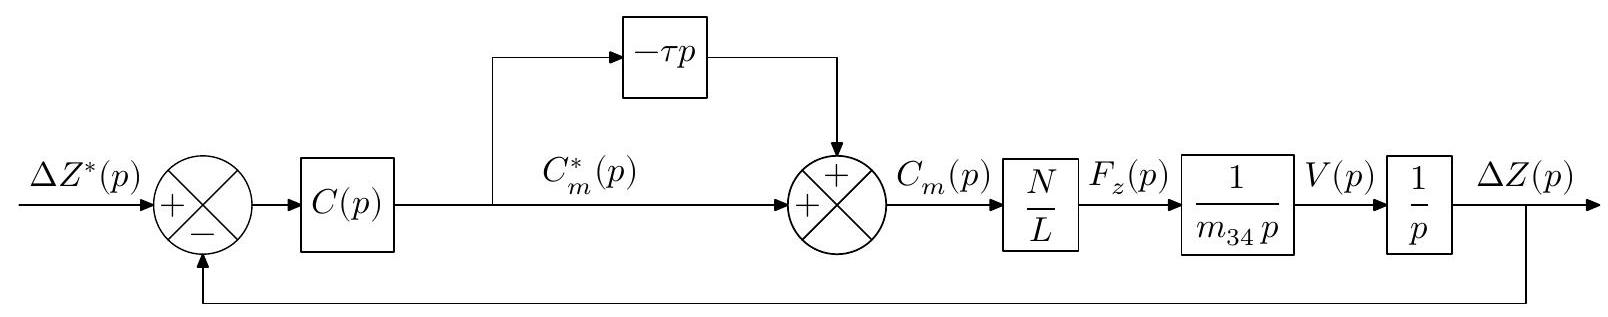
\includegraphics[max width=\textwidth]{2022_12_31_ed674c1a831ea1bff3a0g-09}
\end{center}

Figure $\mathbf{1 1}$ Schéma d'analyse de la robustesse de l'asservissement

Un critère de choix de l'actionneur sera fondé sur une étude de robustesse par rapport à la valeur maximale de ce retard acceptable pour respecter les exigences liées à la stabilité du système.

Dans cette sous-partie, l'effet de la perturbation générée par le poids sur le système n'est pas étudié.

Le système est maintenant étudié en régulation, c'est-à-dire pour lequel l'entrée notée $\Delta Z^{*}(p)=0$. Un schémabloc équivalent est donné (figure 12) en introduisant une entrée virtuelle $W(p)=0$.

\begin{center}
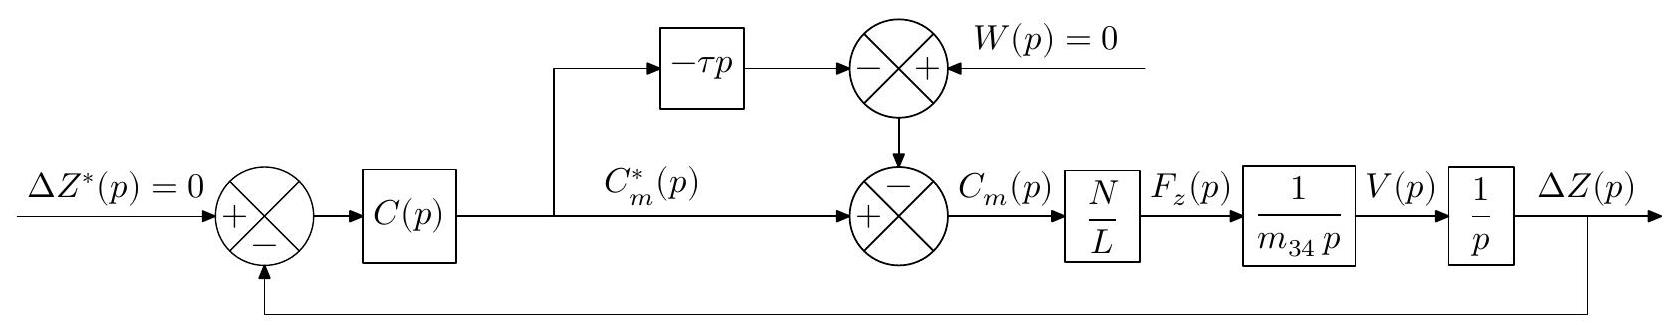
\includegraphics[max width=\textwidth]{2022_12_31_ed674c1a831ea1bff3a0g-09(1)}
\end{center}

Figure 12 Schéma modifié d'analyse de la robustesse de l'asservissement

Q 23. Donner l'expression de la fonction de transfert $H(p)$ présente dans la forme simplifiée du schéma-bloc (figure 13) en fonction de $N, L, m_{34}$ et $C(p)$.

\begin{center}
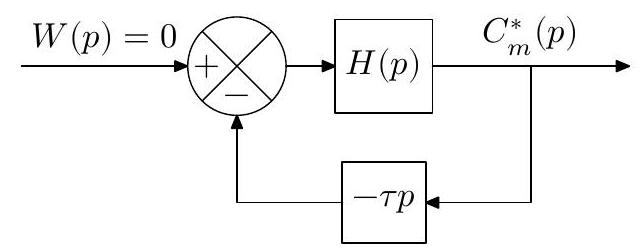
\includegraphics[max width=\textwidth]{2022_12_31_ed674c1a831ea1bff3a0g-09(2)}
\end{center}

Figure 13 Schéma pour l'analyse de la stabilité

En pratique l'action dérivée est filtrée, l'étude du filtrage n'est pas détaillée. Les diagrammes de Bode de la fonction de transfert $H(p)$ ainsi filtrée sont donnés (figure $\mathrm{C}$ du document réponse). Q 24. Compléter ces diagrammes sur le document réponse en représentant les diagrammes de Bode de la fonction $-\tau p$ puis tracer la fonction de transfert en boucle ouverte du système représenté en figure 13 . Pour les tracés, prendre $\tau=1 \mathrm{~s}$ et faire apparaitre clairement les points de construction pour les pulsations $\omega=1 \mathrm{rad} \cdot \mathrm{s}^{-1}$, $\omega=10 \mathrm{rad} \cdot \mathrm{s}^{-1}$ et $\omega=100 \mathrm{rad} \cdot \mathrm{s}^{-1}$.

Q 25. En exploitant le document réponse,

\begin{itemize}
  \item déterminer la valeur de $\tau$ qui assure la stabilité ;

  \item déterminer la valeur de $\tau$ qui assure un amortissement correct en considérant qu'il est obtenu lorsque la marge de phase est d'au moins $60^{\circ}$;

\end{itemize}

— conclure sur une valeur de $\tau$ maximale admissible à spécifier pour le choix du motoréducteur.

\section{IV.C - Conclusion}
Le système est sollicité avec une consigne en échelon d'amplitude $10 \mathrm{~mm}$ à la date $t=1 \mathrm{~s}$. Le graphe représentant l'évolution de $\Delta z^{*}(t)$ et $\Delta z(t)$ est donné pour les deux valeurs extrêmes de masse de l'appareil photo (figure 14).

\begin{center}
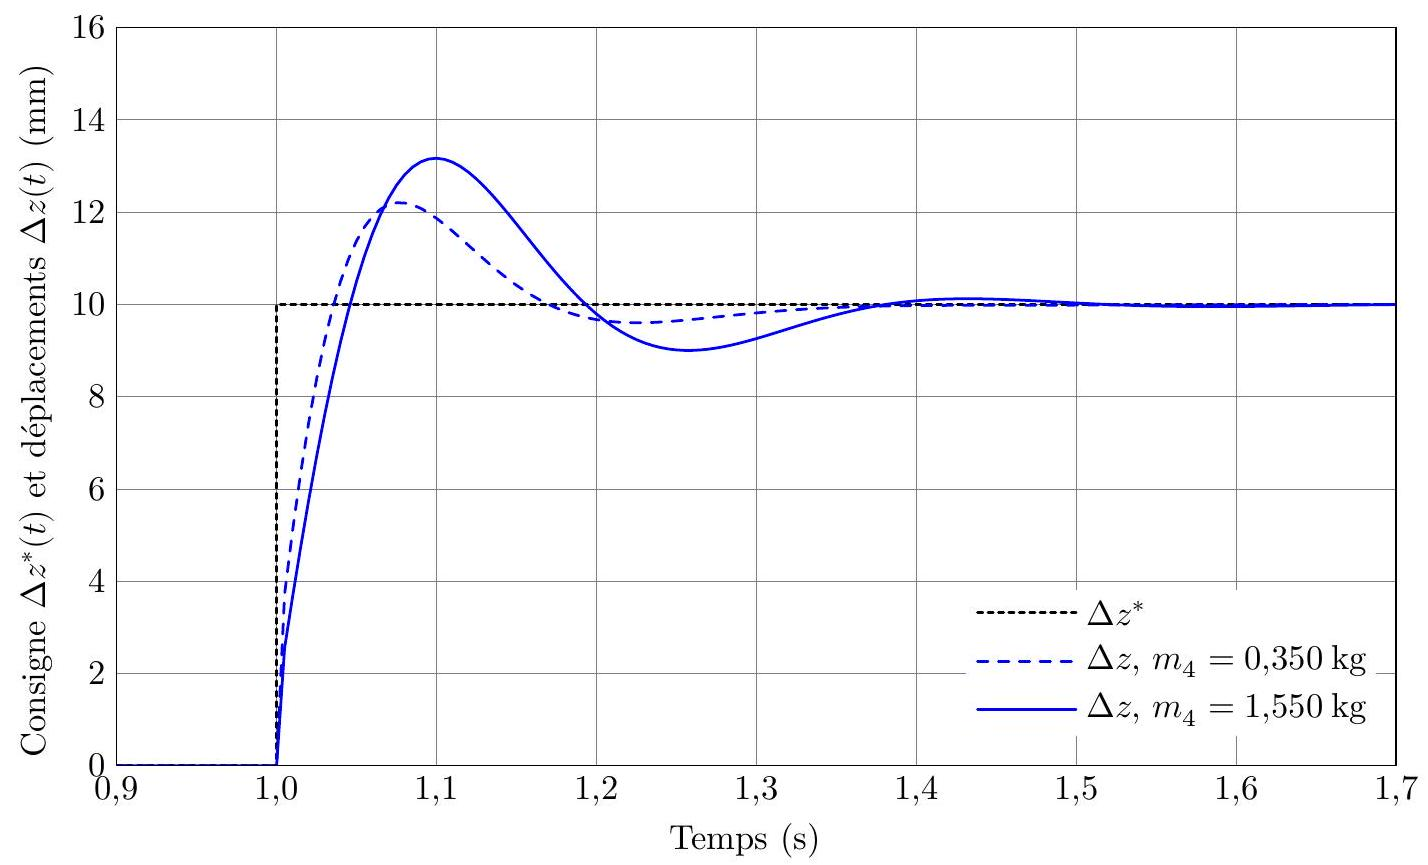
\includegraphics[max width=\textwidth]{2022_12_31_ed674c1a831ea1bff3a0g-10}
\end{center}

Figure 14 Réponse temporelle à un échelon pour les deux valeurs extrêmes de masse de l'appareil photo

Q 26. Conclure sur la capacité du système à satisfaire les exigences du cahier des charges (figure B).

\section{Synthèse}
\section{Objectif}
Analyser et comparer les deux solutions technologiques étudiées précédemment pour concevoir le stabilisateur

Une simulation numérique a été effectuée afin d'analyser la capacité des deux solutions technologiques à vérifier l'exigence 1.2.1 relative au filtrage du mouvement. Pour cela, la réponse harmonique de la fonction $Z_{G}(p) / Z_{\text {pert }}(p)$ obtenue pour le système avec commande active est comparée à celle obtenue avec le système par filtrage passif dont le modèle a été linéarisé (figure 15).

\begin{center}
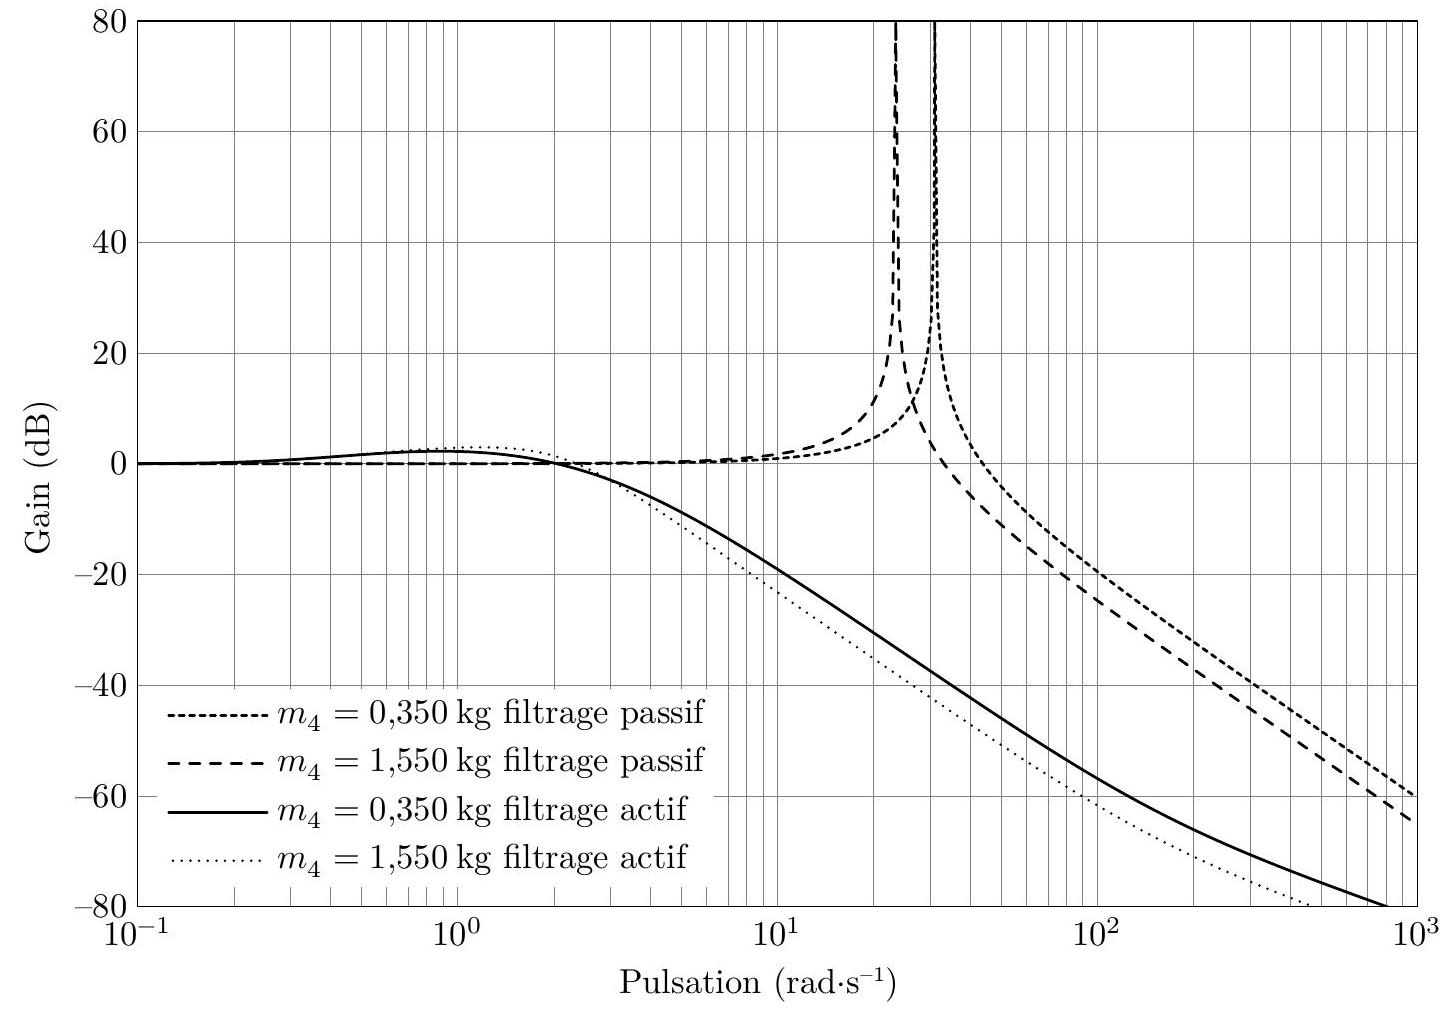
\includegraphics[max width=\textwidth]{2022_12_31_ed674c1a831ea1bff3a0g-11}
\end{center}

Figure 15 Diagrammes de Bode de la fonction $Z_{G}(p) / Z_{\text {pert }}(p)$

Q 27. En étudiant les réponses harmoniques (figure 15), analyser la pertinence de chacune des deux solutions technologiques étudiées à satisfaire l'exigence 1.2.1.

Q 28. En considérant des critères de respect des performances attendues, d'encombrement, de masse, de coût et de consommation d'énergie, établir un tableau comparatif et argumenter un choix entre les deux solutions.

\begin{center}
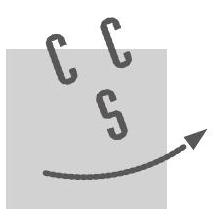
\includegraphics[max width=\textwidth]{2022_12_31_ed674c1a831ea1bff3a0g-12}
\end{center}

Numéro d'inscription

CONCOURS CENTRALE·SUPÉLEC

Numéro de place

Prénom

\begin{center}
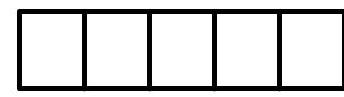
\includegraphics[max width=\textwidth]{2022_12_31_ed674c1a831ea1bff3a0g-12(1)}
\end{center}

Nom

\begin{center}
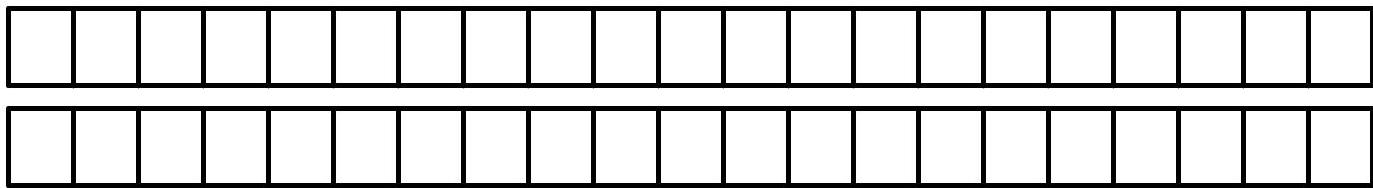
\includegraphics[max width=\textwidth]{2022_12_31_ed674c1a831ea1bff3a0g-12(2)}
\end{center}

ÉpreUVe : Sßl PSI

Ne rien porter sur cette feuille avant d'avoir complètement rempli l'entête

Feville

\begin{center}
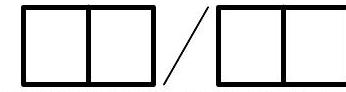
\includegraphics[max width=\textwidth]{2022_12_31_ed674c1a831ea1bff3a0g-12(3)}
\end{center}

Figure A Extrait du cahier des charges fonctionnel

\begin{center}
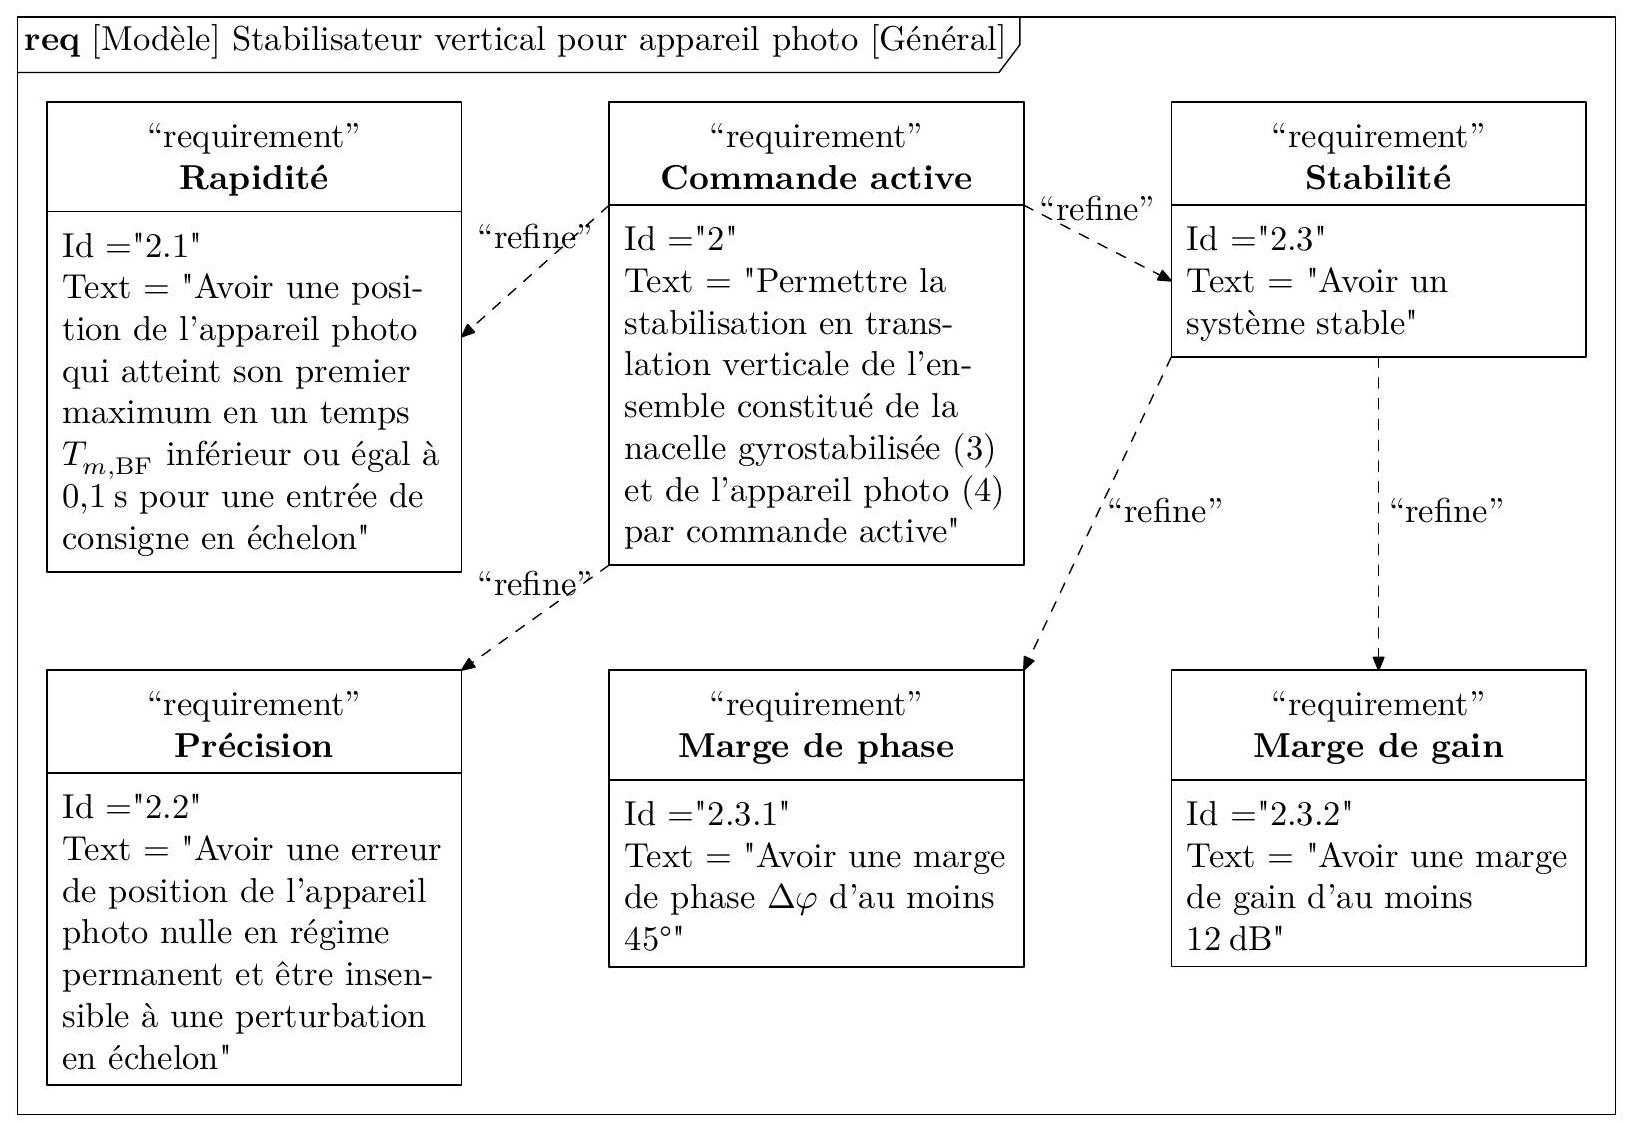
\includegraphics[max width=\textwidth]{2022_12_31_ed674c1a831ea1bff3a0g-13}
\end{center}

Figure B Diagramme des exigences partiel du stabilisateur vertical avec la commande active Questions 24 et 25
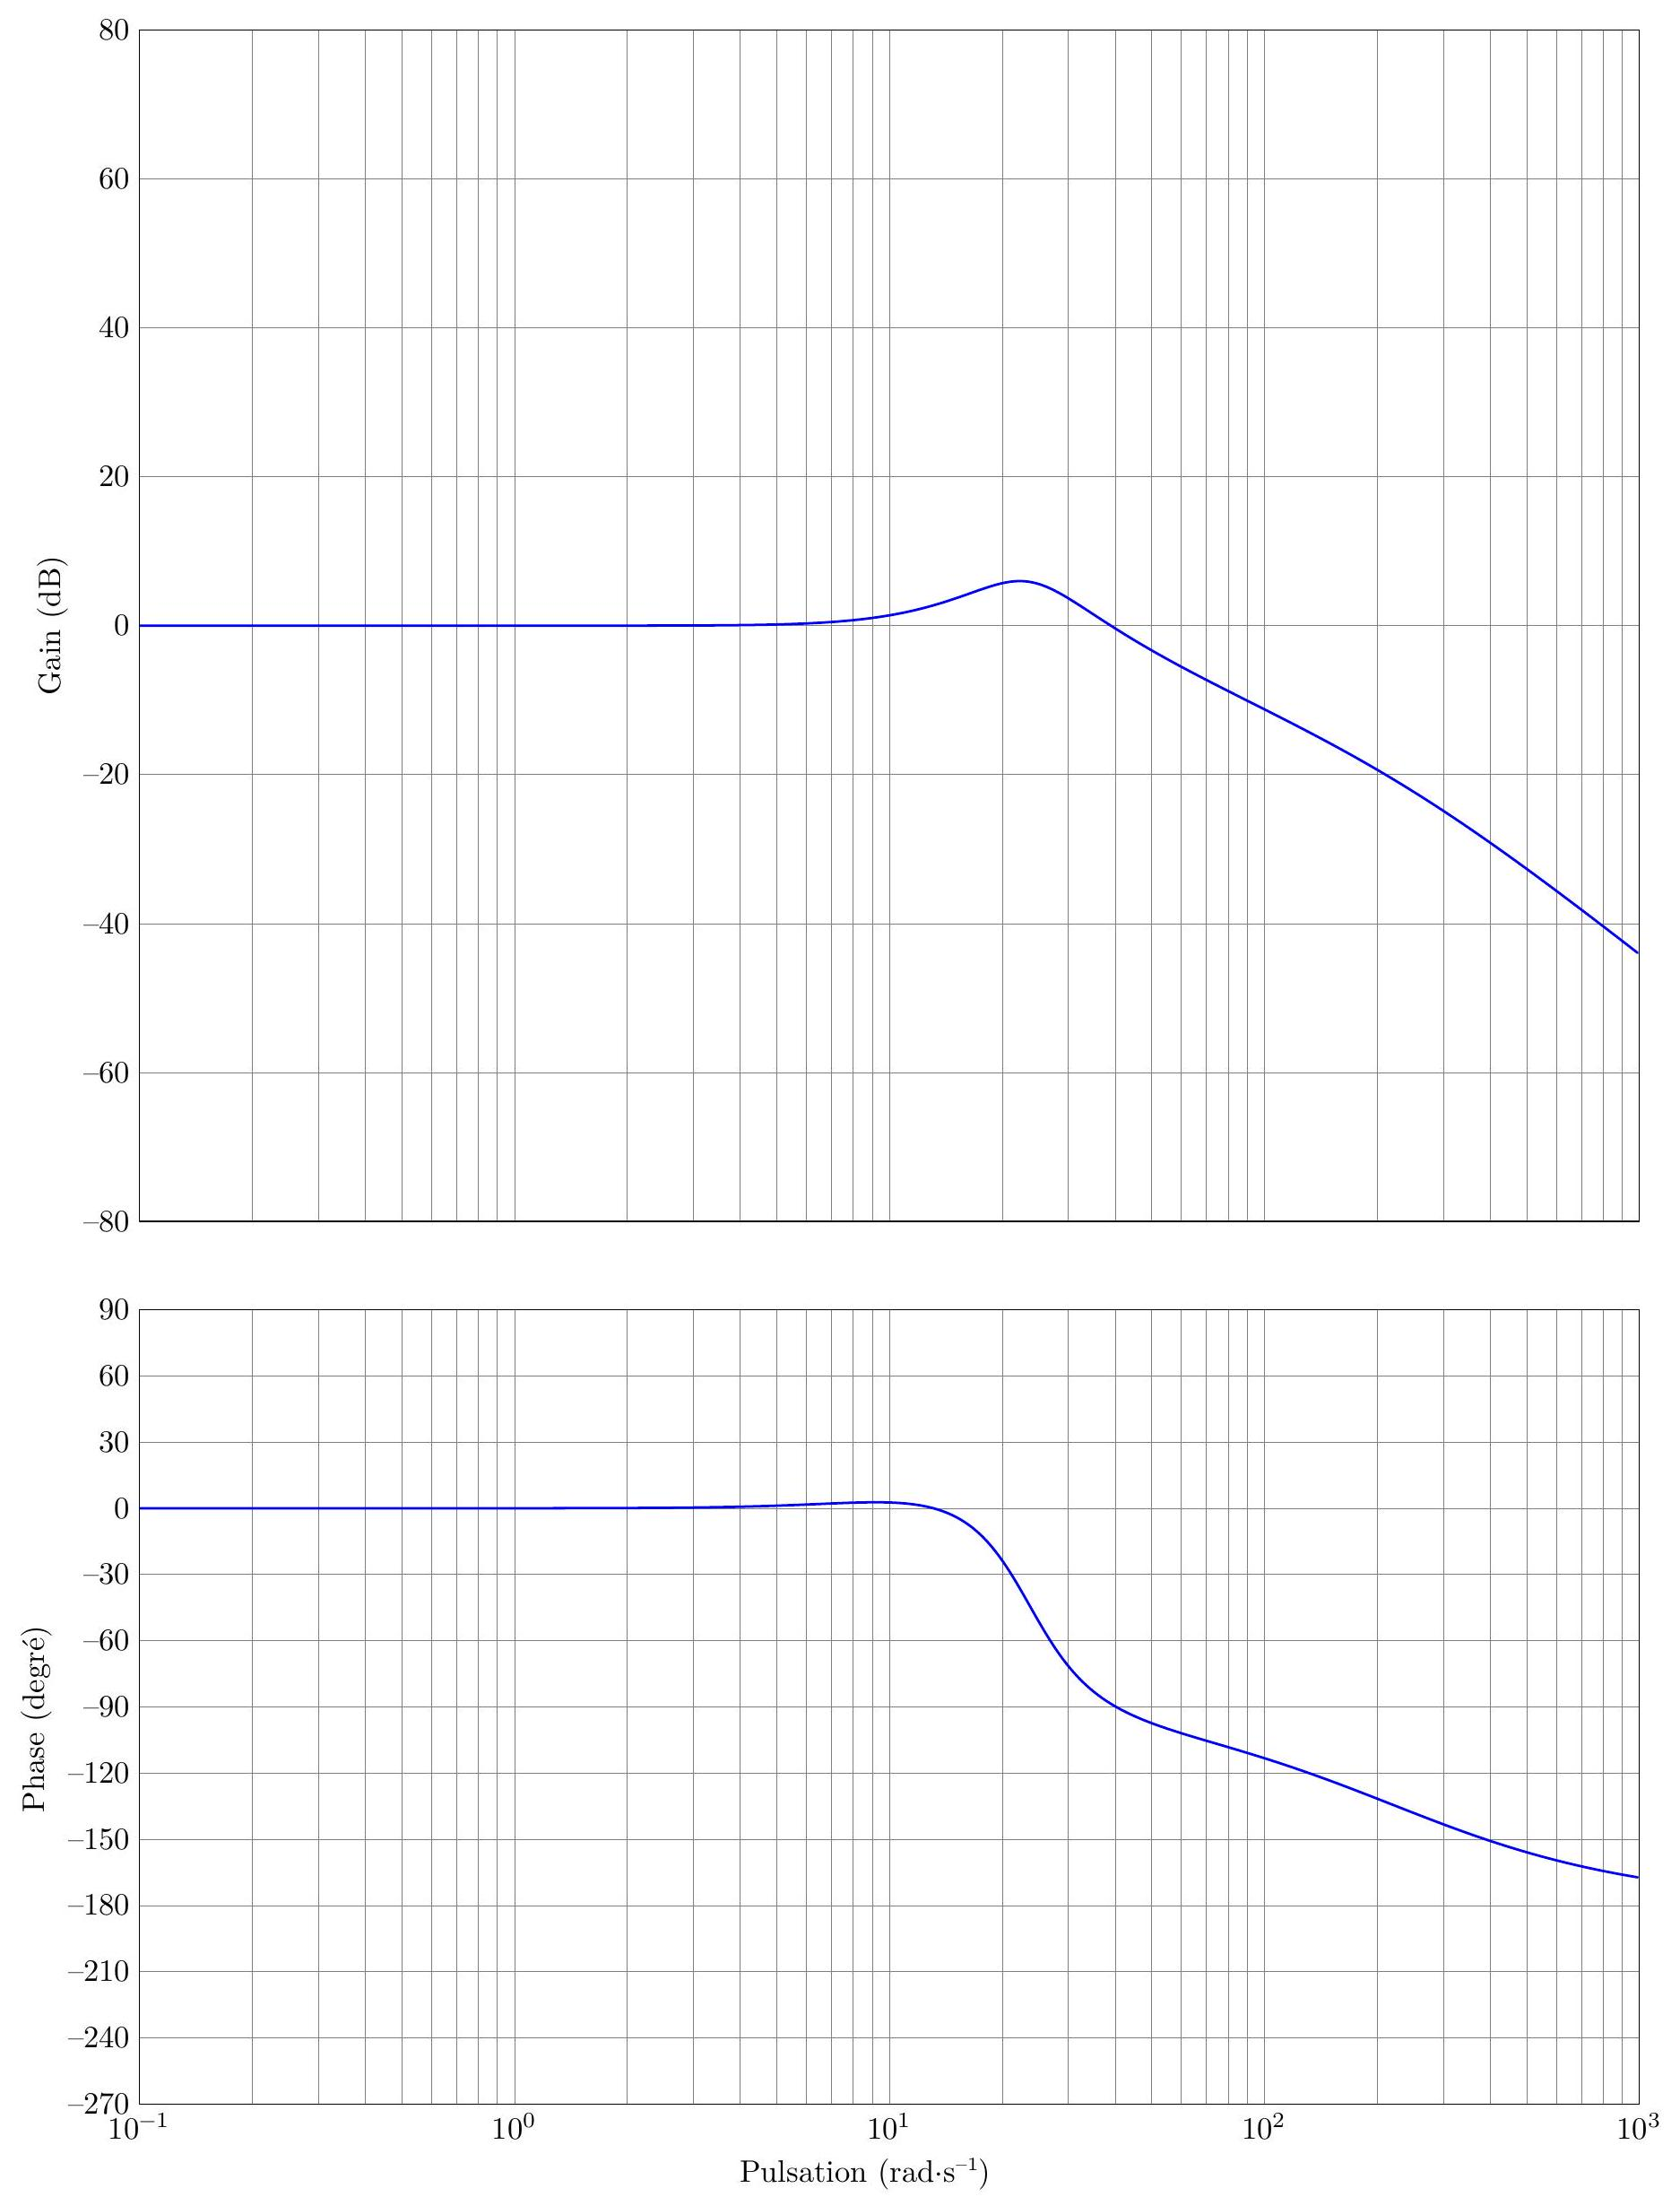
\includegraphics[max width=\textwidth, center]{2022_12_31_ed674c1a831ea1bff3a0g-14}

Figure C Diagrammes de Bode de la fonction $H(p)$ Extrait de l'aide sur la fonction Python scipy.integrate.odeint

\begin{center}
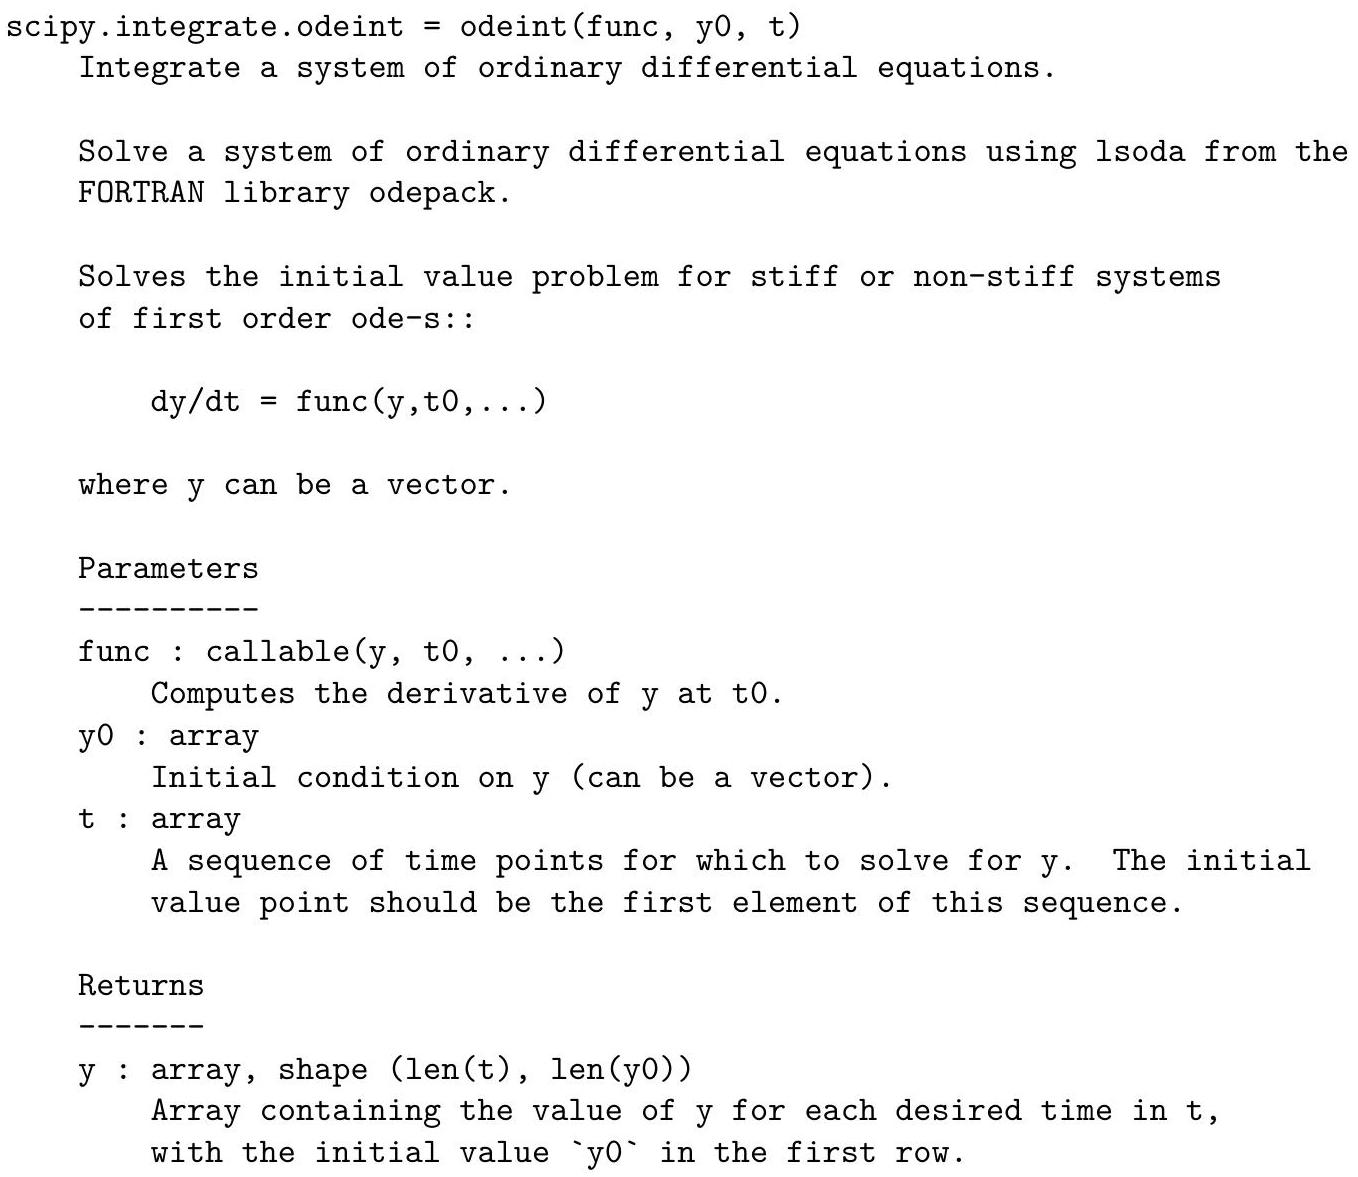
\includegraphics[max width=\textwidth]{2022_12_31_ed674c1a831ea1bff3a0g-15}
\end{center}


\end{document}